%%=============================================================================
%% Methodologie
%%=============================================================================

\chapter{\IfLanguageName{dutch}{Methodologie}{Methodology}}
\label{ch:methodologie}

%% TODO: Hoe ben je te werk gegaan? Verdeel je onderzoek in grote fasen, en
%% licht in elke fase toe welke stappen je gevolgd hebt. Verantwoord waarom je
%% op deze manier te werk gegaan bent. Je moet kunnen aantonen dat je de best
%% mogelijke manier toegepast hebt om een antwoord te vinden op de
%% onderzoeksvraag.

Aan de hand van verchillende RPA providers zal een concreet proces geautomatiseerd worden op Metamaze, het automated document processing platform bij Faktion zelf.


\section{Voorbereiding}
Ter voorbereiding van het te automatiseren proces bij Faktion heb ik mij eerst ingewerkt op het platform waar dit proces zich voordoet. Ook heb ik de volledige 'RPA Developer Essentials' cursus aangeboden door UiPath gevolgd om een algemene basiskennis rond RPA te beheersen. Daarna is de afweging gemaakt welke RPA software providers nu zullen vergelijken worden. Hieruit zijn 5 kandidaten naar boven gekomen. Als 2 grote providers zal gekeken worden naar UiPath en Automation Anywhere. Voor de kleinere providers wordt gekeken naar AutomationEdge en WorkFusion.

Ondertussen werd het te automatiseren proces uitgewerkt. Dit proces zal worden geïmplementeerd op de verschillende  platformen. Het gaat hier over het schrijven van een eigen activiteit die in verschillende workflows kan gebruikt worden om te werken met het Metamaze platform.
\begin{figure}[h]
	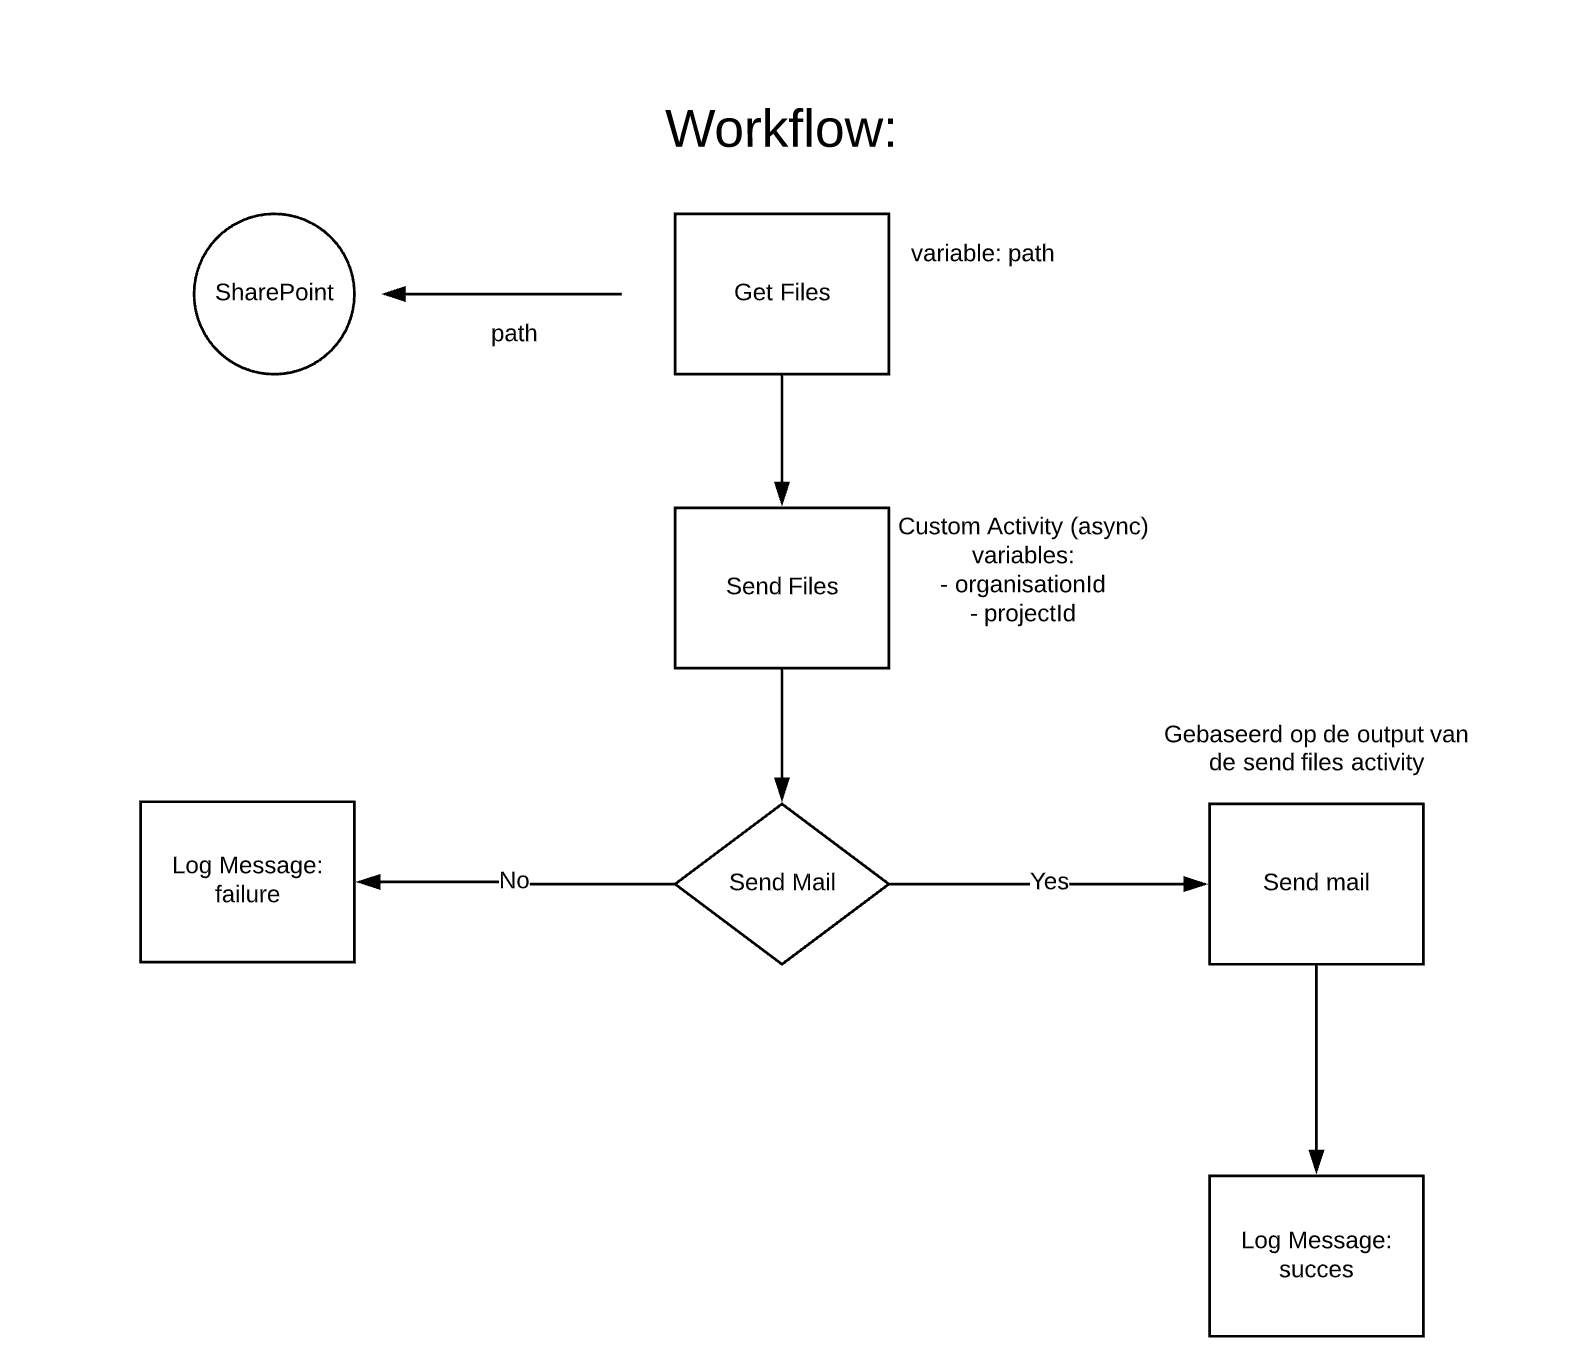
\includegraphics{exampleProcess.png}
	\caption{Voorbeeldproces dat gebruik maakt van de custom Send Files activiteit.}
\end{figure}

\section{Implementatie}
\subsection{UiPath}
\subsection{Automation Anywhere}
\subsection{WorkFusion}
\section{Vergelijking}
